\sectiondate{Figures locales}{}

C’est grâce, en partie, à l’ouvrage collectif « Lozériens connus ou à connaître », que
nous avons pu trouver suffisamment de détails, pour présenter, par ordre alphabétique,
quelques unes de ces personnalités qui ont fait parler d’elles, à Meyrueis même, ou
dans d’autres régions où elles ont vécu et travaillé.

\subsection{Marceline CAUSSE --- 1901-1987}

On ne peut l’évoquer sans voir sa maison de Pradines. Professeur à l’Ecole Normale
de Montpellier, elle a formé aux Sciences Naturelles des générations d’institutrices.
Adhérant au Club Cévenol, elle fit de la section héraultaise une des plus grosses
sections du Club, dit Olivier Poujol : « amenant de nombreux adhérents par le succès des
randonnées pédestres qu’elle reconnaissait scrupuleusement et menait « au sifflet ! » »
Elle a consacré au Club Cévenol une bonne part du dernier tiers de sa vie et elle a justifié le titre du
dernier livre d’A. Chanson : « Il faut vivre vieux ». Mais par son enthousiasme, don tonus, son
amour de la vie, sa sociabilité, sa santé, son entrain qui nous étonnaient, elle justifiait aussi la formule
de Jean Cocteau : « On met longtemps à devenir jeune.

Protestante de vieille roche elle vivait d’une foi sereine et active qui se manifesta
toujours par une générosité financière considérable aussi bien pour son église de la
rue Brueys à Montpellier que pour la Maison de Retraite Protestante de la route de
Ganges où elle finit ses jours et où une salle porte son nom, rappelant son sourire,
son accent et ses exclamations souvent drôles et pointues. !

\subsection{Léon COUDERC --- 1883-1979}

Fils de Louis Couderc, filateur-tisserand, et jeune frère d’Augustine (Grassias) et Emma
(Loupiac). Intelligent, il fut remarqué par Louis Vincent, de la Fabrique, préfet du Nord, qui
l’emmena à Lille pour suivre des études secondaires après lesquelles il entra à l’Institut du
Nord (IDN) d’où il sort ingénieur.
Pendant ses vacances, il obtint, en 1903, l’autorisation d’installer une ligne de téléphone
privée entre le Moulin d’Ayres (la Filature) et sa maison natale au Ferradou, qui était aussi le
magasin de vente sur le chemin du Causse Noir.
Son diplôme d’Ingénieur en poche il fut embauché dans une entreprise de « climatisation » ?
en région parisienne.
Peu satisfait de son travail d’Ingénieur et sensibilisé par la situation des enfants et jeunes en
prison ou en centre de redressement, il fut la cheville ouvrière d’une association d’accueil de
« sortants de prison ». Il fut longtemps directeur d’un de ces foyers d’accueil dans le 20°
arrondissement de Paris. Sa femme, Madeleine de Félice, le seconda très efficacement.

A sa retraite il offrit ses services à l’Eglise Réformée qui l’envoya, comme pasteur
intérimaire à Châtillon sur Loire, Eynesse en Dordogne, Sanary...

\subsection{Raymond FAGES --- 1911-1983}

Fils du pharmacien de Meyrueis, longtemps Maire et Conseiller Général. Après de
brillantes études, il s’investit dans le scoutisme puis s’engagea au service de la
jeunesse catholique de Lozère à qui il a fait découvrir, après la 2\textsuperscript{o} guerre mondiale
les trésors de la Lozère et ceux du monde.
Aumônier de la JAC (Jeunesse Agricole Catholique), il dirigea bien des sessions de
formation rurale, et créa l’école ménagère de Saint Rome de Dolan. Mais c’est
surtout dans l’Hérault qu’il contribuera à la création de plusieurs maisons au service
de l’enfance handicapée :
L’Institut Médico Educatif (IME) de Batipaume , près d’Agde (appelé désormais
Institut Raymond Fages), un autre IME à Florensac et enfin le château de Bellesague
près de Mende qui lui fut offert par la famille du général de la Porte du Theil, ancien
Directeur des Chantiers de Jeunesse.

\subsection{Robert HUBAC --- 1910-1975}

Son père originaire de Conilergues dans la vallée de la Brèze, était pasteur. Agrégé
d’histoire et de géographie, il fut professeur dans les classes de préparation aux
grandes écoles, puis doyen de l’Inspection Générale d’Histoire et de Géographie.
Il pêchait la truite à la mouche, avec adresse aux alentours de sa maison de
Conilergues et me fit remarquer, gentiment, vers 1950, que je pêchais chez lui !
Protestant engagé, il donna bien des articles au journal « Evangile et Liberté », sous
le pseudonyme de Robert Louis (par respect sourilleux de la laïcité).

\subsection{Mgr MARET --- 1805-1884}

Né à Meyrueis, où son père était juge de paix. Doyen de la Faculté de Théologie
Catholique de Paris, il prit parti contre l’absolutisme pontifical, pensant qu’il devait
y avoir un équilibre entre le pouvoir du pape et l’autorité des évêques.
Il ne fut pas écouté et lorsque le dogme de l’Infaillibilité du Pape fut promulgué il se
soumit et dû reprendre à son éditeur tous les exemplaires de son ouvrage exposant
ses idées : « Du concile général et de la paix religieuse ». Pour rembourser ses
dettes, il vendit, sur le Causse Méjean, le domaine de la Calvalade, qu’il avait hérité
de son père.

\subsection{François MARZIALS --- 1779-1861}

Un des derniers pasteurs cévenols formé au Séminaire de Lausanne créé par Antoine
Court, restaurateur des églises protestantes de France. Il fut pasteur à Barnave dans
la Drôme, puis à Nérac et enfin à Montauban. De tendance « évangélique », il fut élu
président du Consistoire de Montauban, à la suite de son collègue et ami Molines,
libéral, qui avait épousé une « héritière-paysanne » de Carnac, près de Rousses, le
village d’origine de la famille Couderc-Loupiac.

\subsection{David POUJOL --- 1870-1939}

Sa famille « sortait » des Oubrets. Après ses études à Montauban, il fut pasteur à
Mazamet pendant de nombreuses années. Très libéral, il faisait preuve d’une
éloquence remarquable, attirant les foules. Cela expliquerait-il, en partie tout au
moins, la naissance d’un petit noyau évangélique rattaché aux Eglises Libres ?
Il perdit un de ses fils à la bataille de la Marne et, très patriote, comme on l’était à
cette époque, donna de nombreuses conférences dans toute la France dans lesquelles
il exaltait le courage de nos troupes face à la barbarie allemande. Ce qui ne laisse pas
de nous étonner aujourd’hui, car on peut penser que l’église dont il était le pasteur,
tout comme les responsables des Eglises Réformées lui laissaient toute liberté !
\emph{(voir son portrait dans « les souvenirs du pasteur Jean Gounelle »)}

\subsection{Frank ROBERT --- 1909 - 1988}

Pasteur de Meyrueis de 1941 à 1946, Frank Robert fut un des responsables de la
résistance à Meyrueis ; il contribua au sauvetage de plusieurs familles juives , de
résistants réfugiés à Meyrueis et ses environs en particulier après l’anéantissement
du maquis Bir Hakeim à la Parade.
Membre du Comité de Libération, il fut adjoint au maire de 1944 et 1945.
Reconnu comme Juste des Nations ( Yad Vaschem à Jérusalem )

\subsection{Rosine ROUEL --- 1881-1902}

Née à Gatuzieres. Après de très brillantes études elle fut nommée à l’âge de 20
ans, directrice du fameux cours complémentaire de filles de Vialas en Lozère.
Malheureusement elle était emportée un an plus tard, sans doute par la tuberculose.

\subsection{Pierre-François SAMUEL, dit « François » --- 1745-1833}

Pasteur de Meyrueis, il est surtout connu par ses prises de position politiques au
moment de la Révolution. Il prend fait et cause pour les Girondins contre
Robespierre : il envoie même une adresse à la Convention contre la tyrannie de la
Montagne. Il essaya de faire passer la Lozère dans le camp des fédéralistes.
Emprisonné, il était en passe de finir sous la guillotine. Mais « ce vigoureux petit
pasteur n’attendit pas, il fit une corde avec ses draps et s’évada, 30 dragons à ses
trousses ».

\emph{(voir les pages : « C’était ça aussi la Révolution à Meyrueis ».}

Il trouva refuge dans le Tarn, avec sa femme et sa fille. Il s’efforça de se justifier
dans une longue lettre et ne fut plus jamais inquiété. Il a été pasteur à Millau et
Puylaurens, ce qui ne l’empêche pas de protester contre les règlements imposant
aux protestants de garnir leurs maisons de tentures lors de la Fête-Dieu, le 2\textsuperscript{o}
dimanche après Pentecôte\footnote{\emph{A la Fête-Dieu, l’hostie sainte, portée en grande pompe dans les rues, était proposée à l’adoration des fidèles catholiques. A Meyrueis, dans les années 1940, les maisons catholiques étaient ornées de draps tendus sur les façades, ainsi que de reposoirs avec des bouquets, des décorations, des images pieuses, pour le passage de la procession.}}.

\subsection{Robert VERDIER --- 1910 -- 2009}

Retrouve sa maison de Pont Vieux tous les étés car il a de solides attaches à
Meyrueis :

\begin{quote}
\emph{« mon arrière grand-père originaire de Cabrillac s’était marié à Meyrueis. Sabotier
et cultivateur, ardent républicain il inculqua ses valeurs à toute la famille. Jaurès
était l’homme à suivre ».}
\end{quote}

Après une agrégation de lettres classiques, il est nommé au Lycée Carnot en 1937. Il
fonde le Comité d’Action Socialiste qui deviendra le Parti Socialiste clandestin
pendant les années d’occupation. : \emph{« J’éprouve toujours beaucoup d’émotion
lorsqu’on évoque la mémoire de mes camarades morts en déportation : Pierre
Brossolette, Roger Bouvet et bien d’autres... ».}

Plus tard dans les années 1960, Robert Verdier prend part avec Alain Savary à la
création du PSU. Et c’est grâce à Alain Savary, devenu ministre de l’Education
Nationale, que fut « sauvé » le collège d’enseignement général de Meyrueis
condamné à cause de la faiblesse de ses effectifs. Il put disposer des nouveaux
locaux que nous connaissons aujourd’hui et fut baptisé Collège André Chanson.

% Illustration : Meyrueis, 1890.
% La photographie sera remplacée ultérieurement par une image restaurée.

\begin{center}
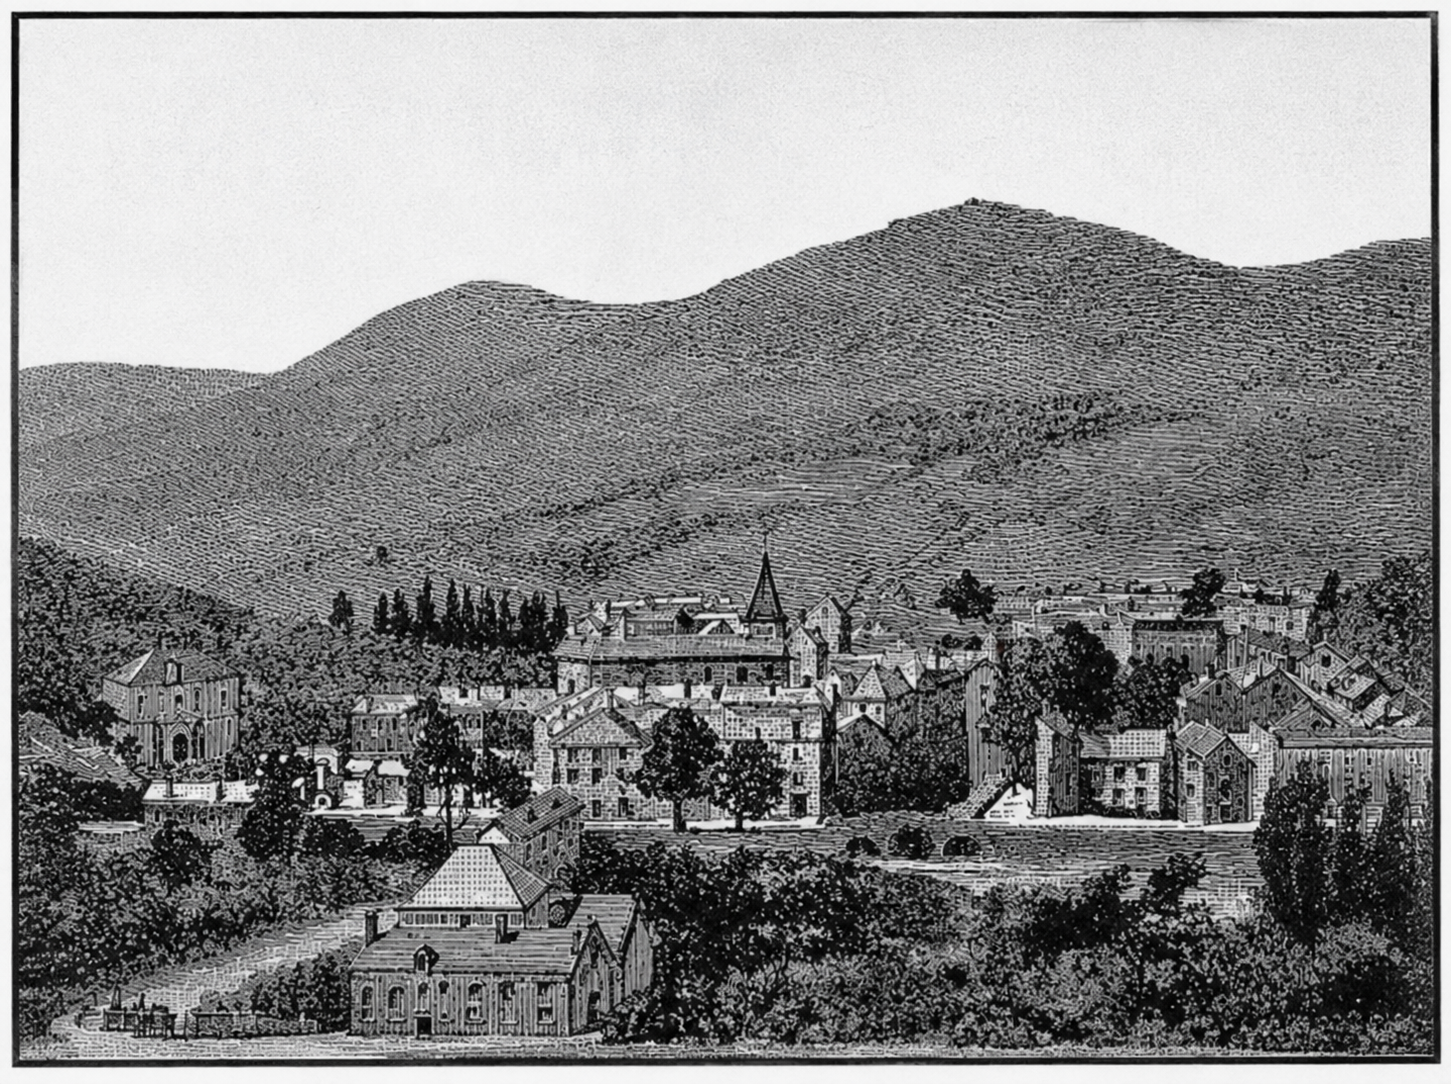
\includegraphics[width=0.60\textwidth]{imgs/132}\\
\emph{Meyrueis. 1890.}
\end{center}
